\chapter{Event Selection}

\label{ch:selection}

The \acp{LLP} targeted by this search differ in their interactions with the detector from \ac{SM} particles primarily because of their large mass. 
When produced at the energies available at the \ac{LHC}, that large mass results in a low $\beta$ (typically $0.2 < \beta < 0.9$). 
Such slow-moving particles heavily ionize in detector material. 
Each layer of the pixel detector provides a measurement of that ionization, through \ac{ToT}, as discussed in Section~\ref{sec:pixel_dedx}. 
The ionization in the pixel detector, quantified in terms of \dedx, provides the major focus for this search technique, along with the momentum measured in the entire inner detector.
It is effective both for its discriminating power and its use in reconstructing a particle's mass, and it can be used for a wide range of masses and lifetimes as discussed in Section~\ref{sec:rh_lifetimes}. 
However \dedx needs to be augmented with a few additional selection requirements to provide a mechanism for triggering and to further reduce backgrounds.

Ionization itself is not currently accessible for triggering, so this search instead relies on \met to trigger signal events.
Although triggering on \met can be inefficient, \met is often large for many production mechanisms of \acp{LLP}, as discussed in Section~\ref{sec:characteristics}.

The use of ionization to reject \ac{SM} backgrounds relies on well-measured, high-momentum tracks, so some basic requirements on quality and kinematics are placed on the tracks considered in this search. 
These quality requirements have been significantly enhanced in Run 2 by a newly introduced tracking variable that is very effective in removing highly-ionizing backgrounds caused by overlapping tracks. 
A few additional requirements are placed on the tracks considered for \ac{LLP} candidates that increase background rejection by targeting specific types of \ac{SM} particles. 
These techniques provide a significant analysis improvement over previous iterations of ionization-based searches on ATLAS by providing additional background rejection with minimal loss in signal efficiency. 

The ionization measurement with the Pixel detector can be calibrated to provide an estimator of $\beta\gamma$. That estimate, together with the momentum measurement provided by tracking, can be used to reconstruct a mass for each track which traverses the pixel detector. 
That mass variable will be peaked at the \ac{LLP} mass for any signal, and provides an additional tool to search for an excess.
In addition to an explicit requirement on ionization, this search constructs a mass-window for each targeted signal mass in order to evaluate any excess of events and to set limits. 
%Construction, calibration, and requirements for the mass variable are discussed in Section~\ref{sec:mass_requirement}.

The strategy discussed here is optimized for lifetimes of $O(1)$ - $O(10)$ ns. 
Pixel ionization is especially useful in this regime as particles only need to propagate through the first seven layers of the inner detector, about 37 cm from the beam axis. 
The search is still competitive with other searches for \acp{LLP} at longer lifetimes, because the primary discriminating variables are still applicable even for particles that do not decay within the detector~\cite{stable2016}. 
Although the majority of the requirements will be the same for all lifetimes, two signal regions are defined to optimize separately for intermediate and long lifetime particles.


% --------------------------------------------------------------------------------

\section{Trigger}

Triggering remains a significant difficulty in defining an event selection with high signal efficiency in a search for \acp{LLP}. 
There are no triggers available in the current ATLAS system that can fire directly from a high momentum track with large ionization (Section~\ref{sec:trigger}). 
Although in some configurations a charged \ac{LLP} can fire muon triggers, this requirement introduces significant model dependence on both the allowed lifetimes and the interactions in the calorimeter~\cite{rhad_atlas}, as discussed in Section~\ref{sec:rh_interactions}.

For a search targeting particles which may decay prior to reaching the muon system, the most efficient available trigger is based on missing energy~\cite{rhad_atlas}.
As discussed in Section~\ref{sec:characteristics}, signal events can produce significant \met by a few mechanisms.
At the trigger level however, the missing energy is only calculated using the calorimeters (Section~\ref{sec:trigger}) where the \rhadrons deposit little energy.
So, at short lifetimes, \met measured in the calorimeter is generated by an imbalance between the jets and undetected \acp{LSP} produced in \rhadron decays.
At longer lifetimes, without the decay products, missing energy is only produced in the calorimeters when the \rhadrons recoil against an \ac{ISR} jet.

These features are highlighted in Figure~\ref{fig:trigger_met}, which shows the \met distributions for simulated short lifetime (3 ns) and stable \rhadron events.
The figure includes both the offline \met, the missing energy calculated with all available information, and \calomet, the missing energy calculated using only information available at the calorimeter which approximates the missing energy available at the trigger.
The short lifetime sample has significantly greater \met and \calomet than the stable sample as expected.
For the stable sample, a small fraction of events with very large \met (about 5\%) migrate into the bin with very small \calomet because the \met produced by a charged \rhadron track opposite a neutral \rhadron track does not contribute any missing energy in the calorimeters.

\begin{figure}[h]
\centering
\subfloat[]{
  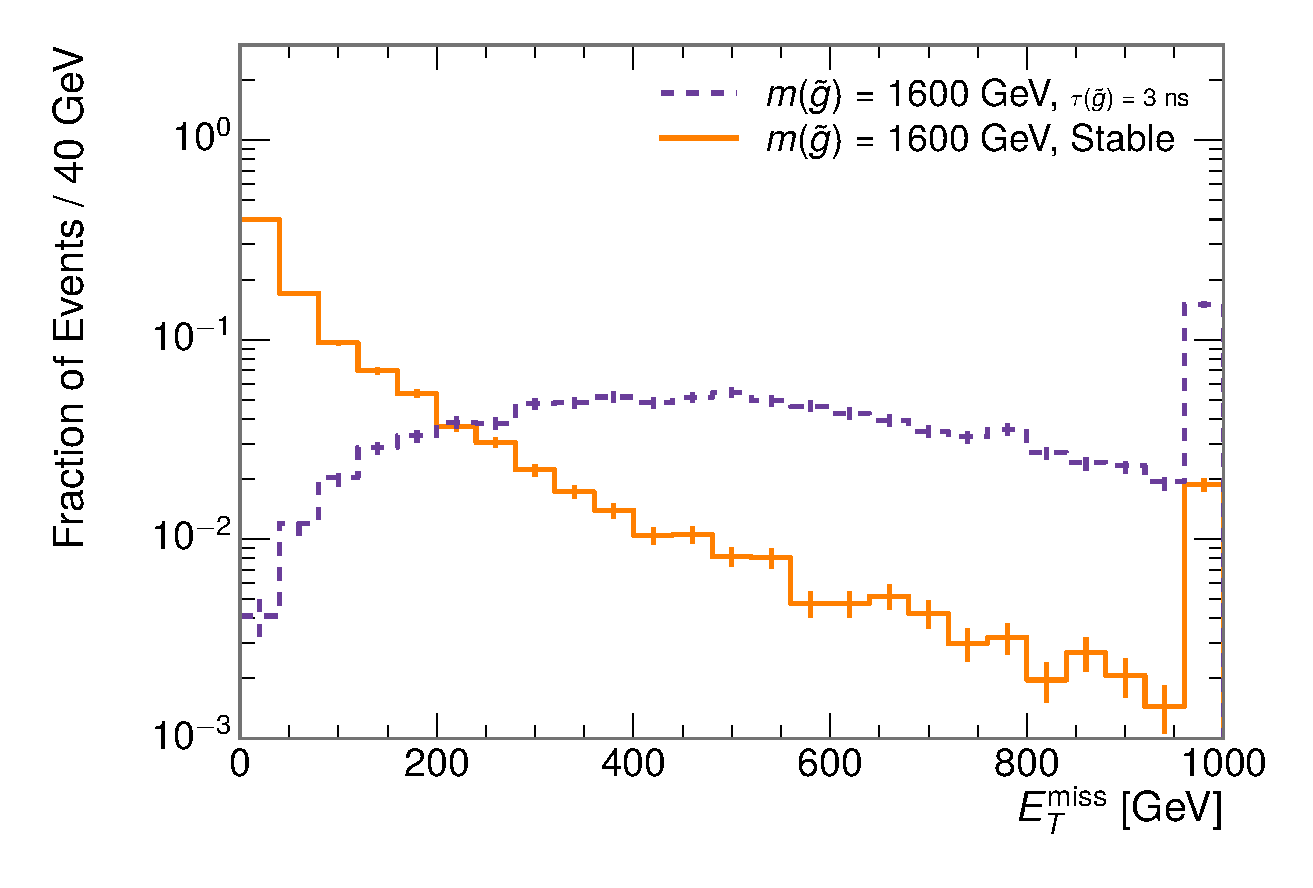
\includegraphics[width=\halffig]{figures/trigger_met.pdf}
}
\subfloat[]{
  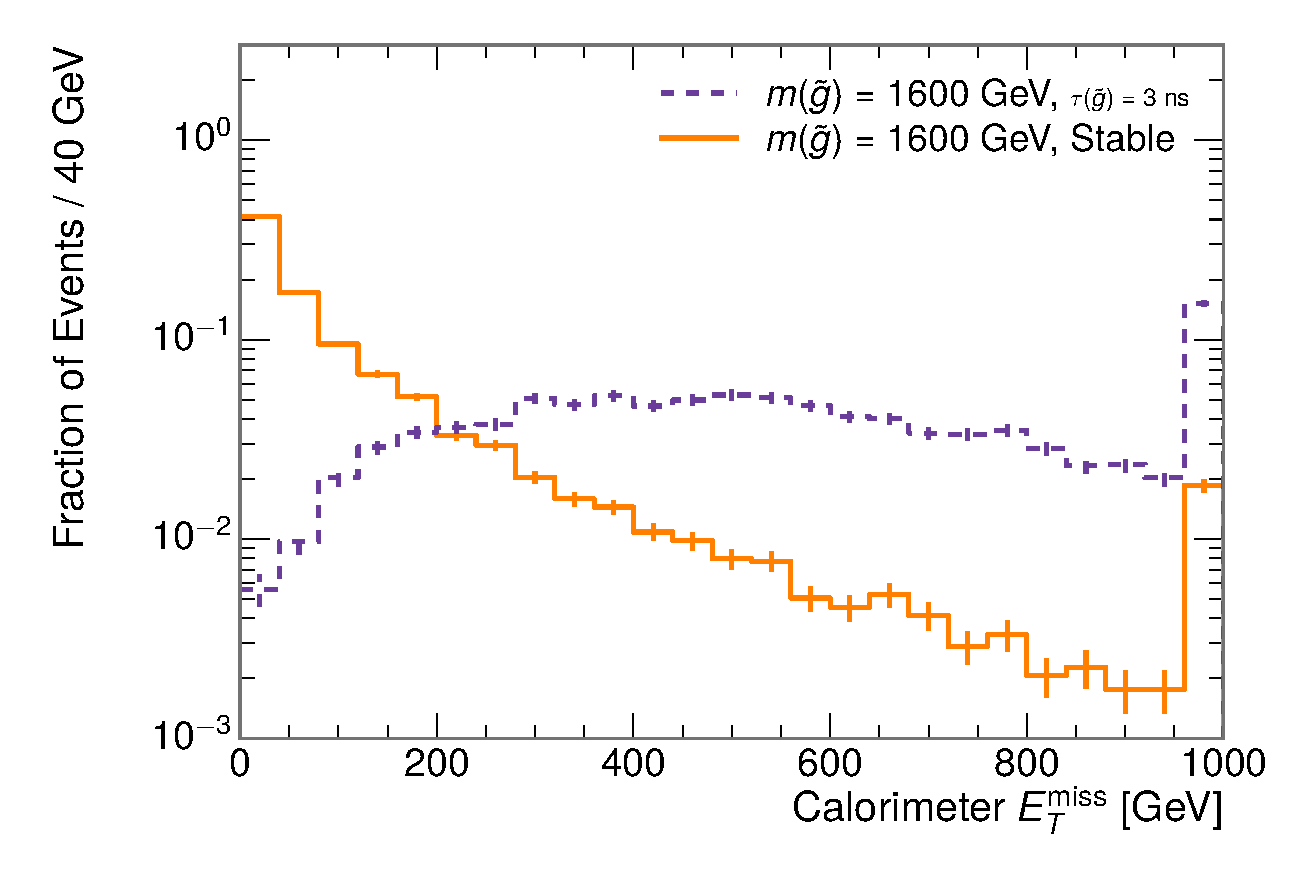
\includegraphics[width=\halffig]{figures/trigger_calomet.pdf}
}
\caption{The distribution of (a) \met and (b) \calomet for simulated signal events before the trigger requirement.}
\label{fig:trigger_met}
\end{figure}

So, either case to some extent relies on kinematic degrees of freedom to produce missing energy, as the pair-produced \acp{LLP} tend to balance each other in the transverse plain.
That balance results in a relatively low efficiency for long-lifetime particles, roughly 40\%, and efficiencies between 65\% and 95\% for shorter lifetimes depending on both the mass and the lifetime.
For long lifetimes in particular, the presence of \ac{ISR} is important in providing an imbalance in the transverse plane, and is an important aspect of modeling the selection efficiency for \rhadron events.

The missing energy trigger with the lowest threshold available is chosen for this selection in order to maximize the trigger efficiency. 
During 2015 data collection this was the \texttt{HLT\_xe70} trigger, which used a 50 \GeV threshold on missing energy at \texttt{LVL1} and a 70 \GeV threshold on missing energy at the \texttt{HLT}.
These formation of the trigger decision for missing energy was discussed in more detail in Section~\ref{sec:trigger}.


% ----------------------------------------

\section{Kinematics and Isolation}
\label{sec:track_requirements}

After the trigger requirement, each event is required to have a primary vertex reconstructed from at least two well-measured tracks in the inner detector, each with $\pt > 400$ \MeV. 
If more than one such vertex exists, the primary vertex is taken to be the one with the largest summed track momentum for all tracks associated to that vertex. 
The offline reconstructed \met is required to be above 130 \GeV to additionally reject \ac{SM} backgrounds.
The transverse missing energy is calculated using fully reconstructed and calibrated offline objects, as described in Section~\ref{sec:missing_energy}. 
In particular the \met definition in this selection uses jets reconstructed with the anti-$k_t$ algorithm with radius $R = 0.4$ from clusters of energy in the calorimeter (Section~\ref{sec:jets}) and with $p_T > 20$ \GeV, as well as reconstructed muons, electrons, and tracks not identified as another object type.

The \met distributions are shown for data and a few simulated signals in Figure~\ref{fig:nm1_met}, after the trigger requirement.
The cut placed at 130 \GeV is 95\% efficient for metastable and 90\% efficient for stable particles, after the trigger requirement, because of the missing energy generating mechanisms discussed previously.
The distribution of data in this figure and subsequent figures in this section can be interpreted as the distribution of backgrounds, as any signal contamination would be negligible if present at these early stages of the selection (prior to the final requirement on ionization). 
The background falls rapidly with missing energy, motivating the direct requirement on \met for the signal region.
Although a tighter requirement than the specified value of 130 \GeV would seem to increase the search potential from these early distributions, other requirements are more optimal when taken as a whole.
The specific values for each requirement in signal region were optimized considering the increase in discovery reach for tightening the requirement on each discriminating variable. 
\textbf{NOTE: If space and time permit, I will add a whole section about signal region optimization..}

\begin{figure}[h]
\centering
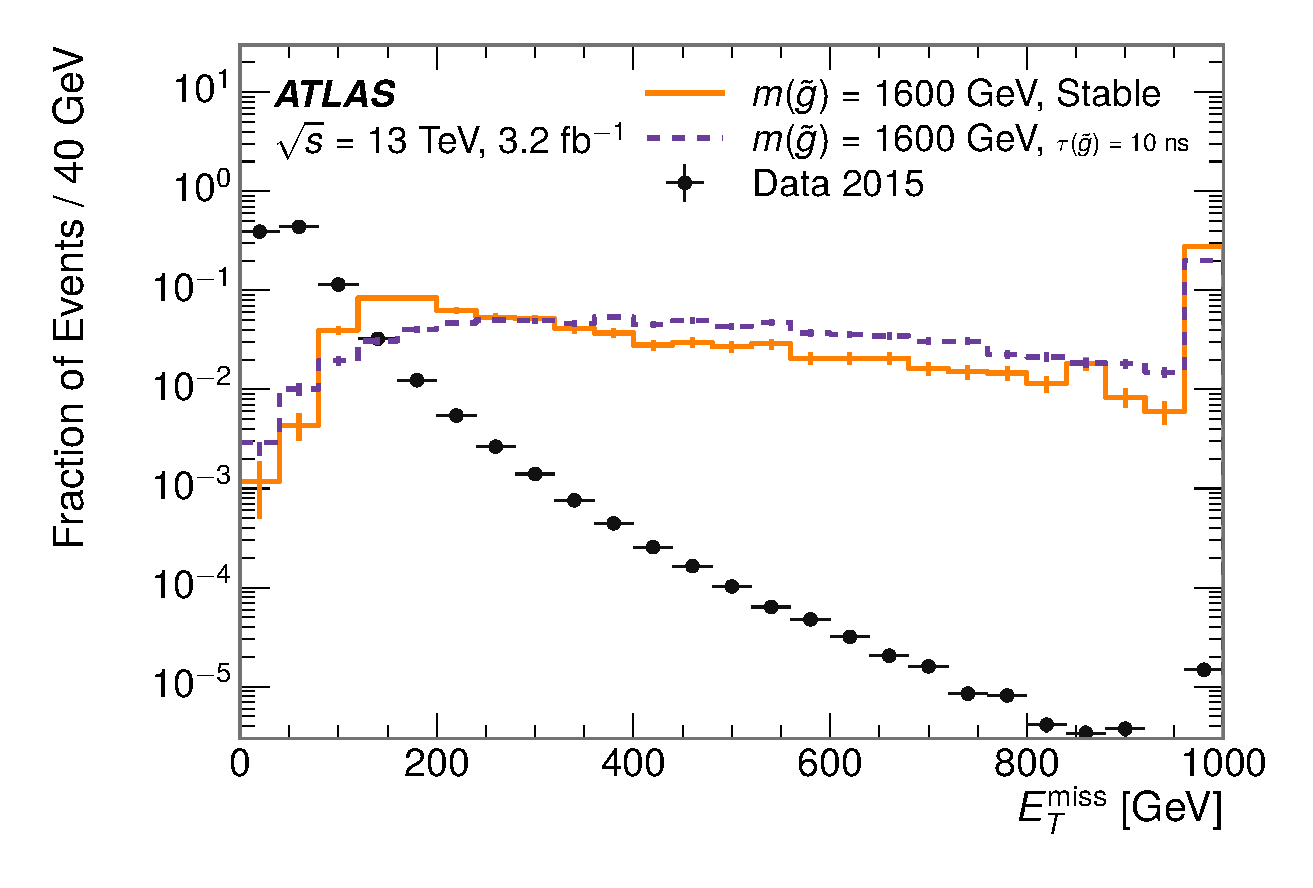
\includegraphics[width=\fullfig]{figures/selection_met_nm1_log.pdf}
\caption{The distribution of \met for data and simulated signal events, after the trigger requirement.}
\label{fig:nm1_met}
\end{figure}

It is typically the practice for searches for new physics on \ac{ATLAS} to place an offline requirement on the triggering variable that is sufficiently tight to guarantee that the event would pass the trigger.
Such a tight requirement makes the uncertainty on the trigger efficiency of the simulation negligible, as modeling the regime where the trigger is only partially efficient can be difficult.
In this analysis, however, because of the atypical interactions of \rhadrons with the tracker and the calorimeter, the offline requirement on \met is not sufficient to guarantee a 100\% trigger efficiency even at large values, as can be seen in Figure~\ref{fig:trigger_turnon}.
This figure shows the efficiency for passing the \texttt{HLT\_xe70} trigger as a function of the requirement on \met, which plateaus to roughly 85\% even at large values.
This plateau does not reach 100\% because events which have large offline missing energy from a neutral \rhadron produced opposite of a charged \rhadron can have low missing energy in the calorimeters.
The \calomet, on the other hand, does not have this effect and reaches 100\% efficiency at large values because it is the quantity that directly corresponds to the trigger threshold.
In both cases the efficiency of triggering is greater for the short lifetime sample because the late decays to hadrons and \acp{LSP} produce an imbalance in the calorimeters even though they may not be reconstructed offline as tracks or jets.
For this reason, the requirement on \met is determined by optimizing the background rejection even though it corresponds to a value of trigger efficiency significantly below 1.0.

\begin{figure}[h]
\centering
\subfloat[]{
  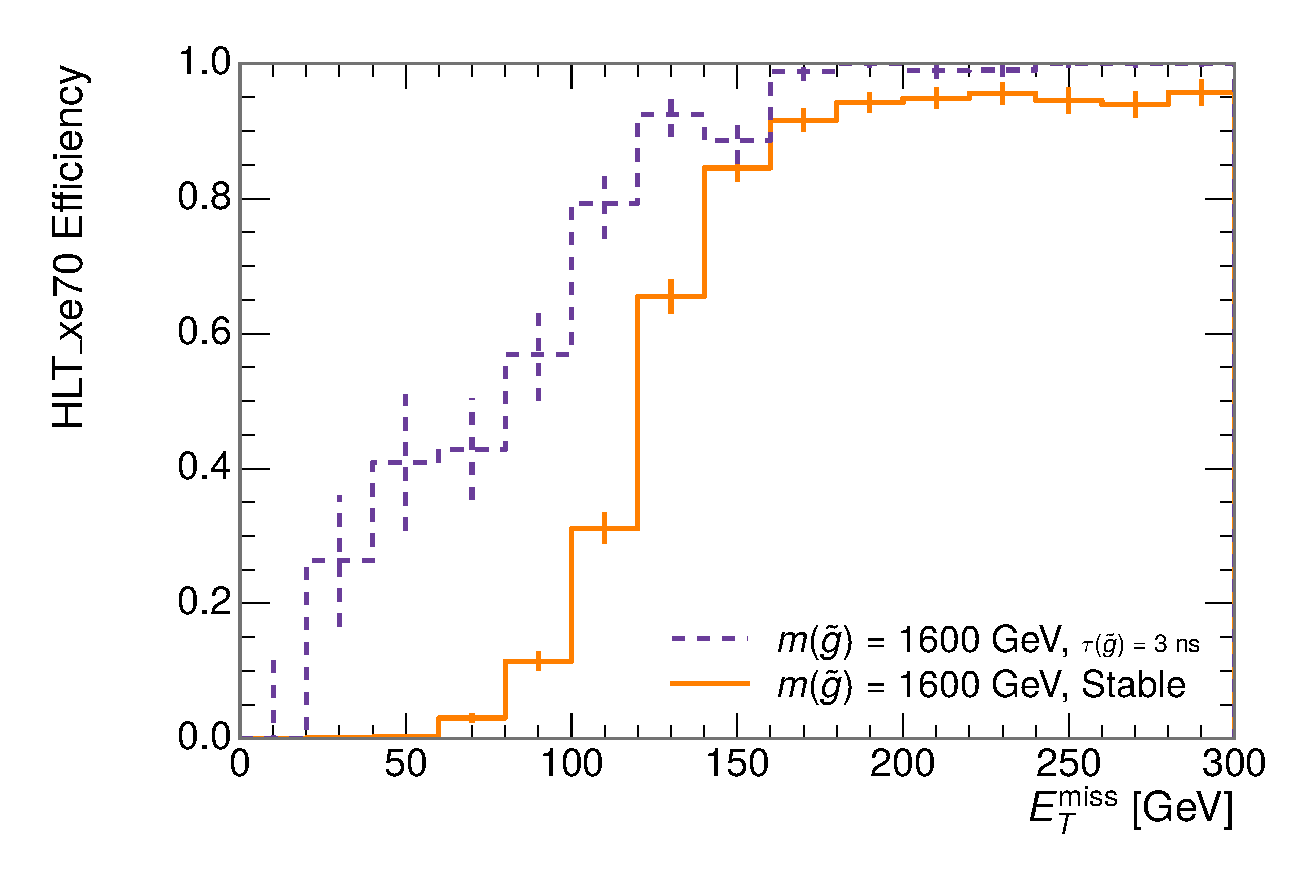
\includegraphics[width=\halffig]{figures/teff_met_signal.pdf}
}
\subfloat[]{
  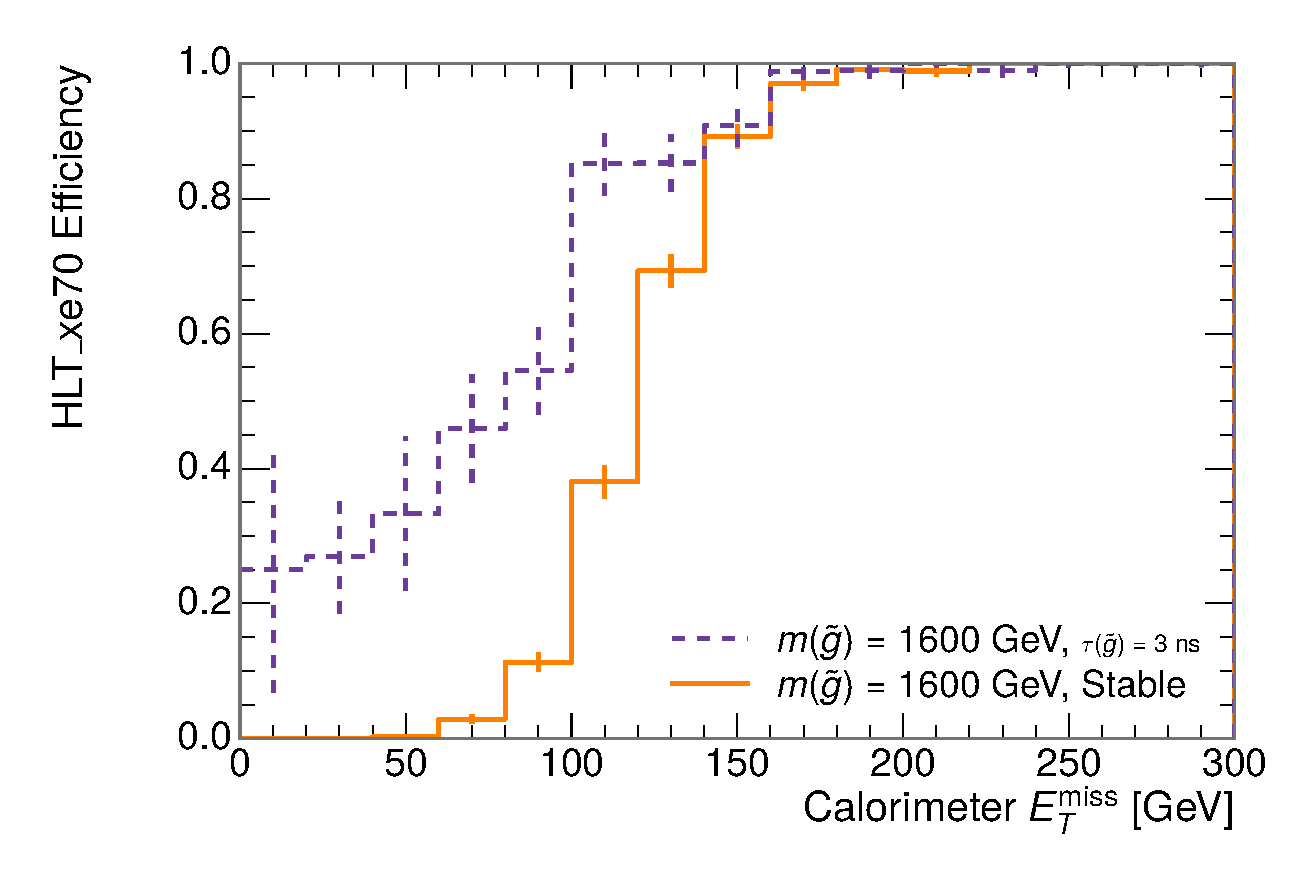
\includegraphics[width=\halffig]{figures/teff_calomet_signal.pdf}
}
\caption{The trigger efficiency for the \texttt{HLT\_xe70} trigger requirement as a function of (a) \met and (b) \calomet for simulated signal events.}
\label{fig:trigger_turnon}
\end{figure}

Potential signal events are then required to have at least one candidate \ac{LLP} track.
Although the \acp{LLP} are produced in pairs, many models do not consistently yield two charged particles.
For example, in the \rhadron model highlighted here, only 20\% of events have two charged \rhadrons while 47\% of events have just one.
A signal region requiring two charged candidates could be a powerful improvement in background rejection for a larger dataset, but it is not considered in this version of the analysis as it was found to be unnecessary to reject the majority of backgrounds.

For a track to be selected as a candidate, it must have $p_T > 50$ \GeV and pass basic quality requirements. 
The track must be associated to the primary vertex.
It must also have at least seven clusters in the silicon layers in the inner detector to ensure an accurate measurement of momentum.
Those clusters must include one in the innermost layer if the extrapolated track is expected to pass through that layer.
And to ensure a reliable measurement of ionization, the track is required to have at least two clusters in the pixel detector that provide a measurement of \dedx.

At this point in the selection, there is a significant high-ionization background from multiple tracks that significantly overlap in the inner detector. 
Previous version of this analysis have rejected these overlaps by an explicit overlap rejection between pairs of fully reconstructed tracks, typically by requiring no additional tracks within a cone around the candidate. 
This technique, however, fails to remove the background from tracks that overlap so precisely that the tracks cannot be separately resolved, which can be produced in very collimated photon conversions or decays of pions.

A new method, added in Run 2, identifies cluster shapes that are likely formed by multiple particles based on a neural network classification algorithm.
The number of clusters that are classified this way in the pixel detector for a given track is called \Nsplit.
As the shape of clusters requires significantly less spatial separation to identify overlaps than it does to reconstruct two fully resolved tracks, this variable is more effective at rejecting backgrounds from overlaps.
Figure~\ref{fig:dedx_nsplit} shows the dependence of ionization on \Nsplit; as \Nsplit increases the most probable value of \dedx grows significantly up to twice the expected value when $\Nsplit = 4$. 

\begin{figure}[h]
\centering
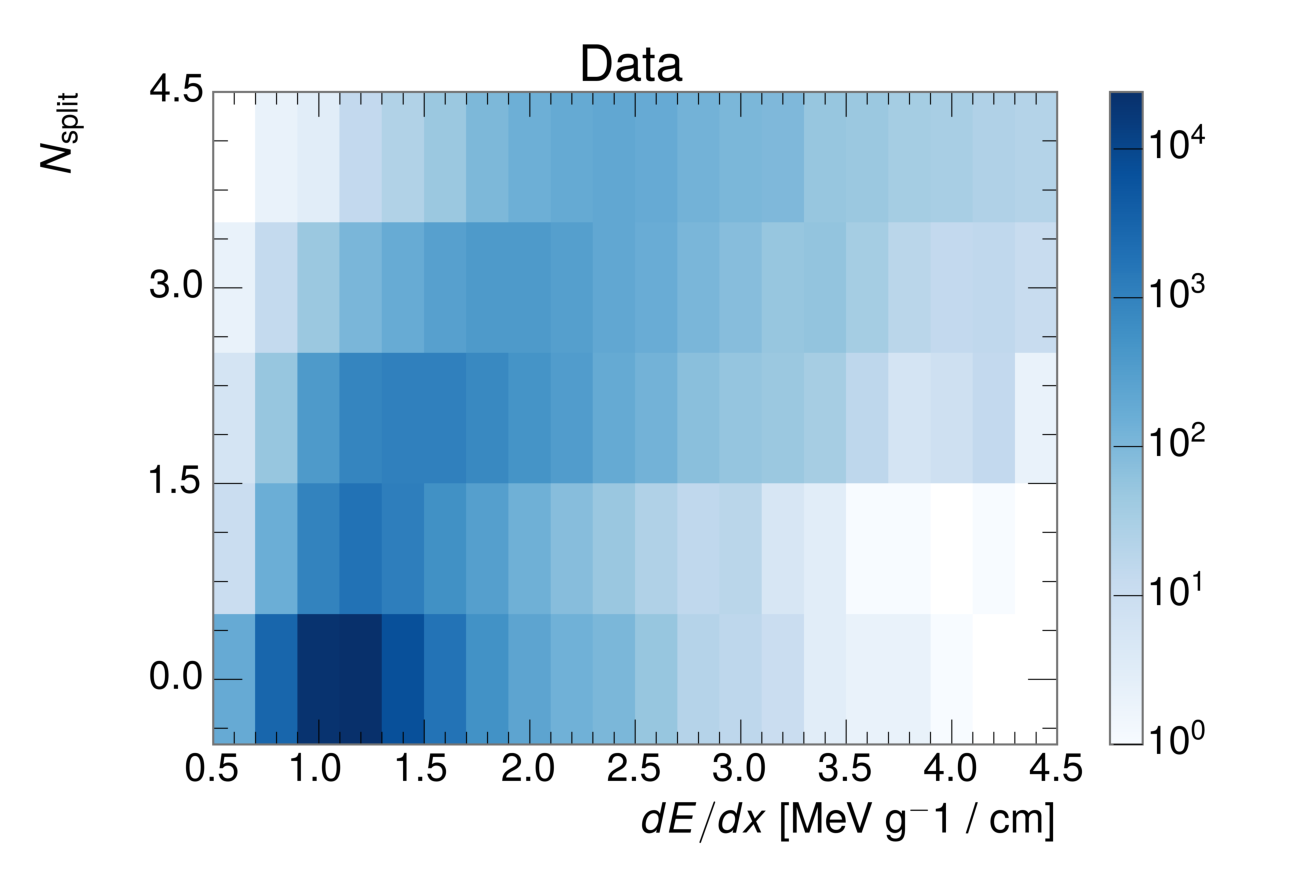
\includegraphics[width=\fullfig]{figures/dedx_nsplit_data.pdf}
\caption{The dependence of \dedx on $N_{\mathrm{split}}$ in data after basic track hit requirements have been applied.}
\label{fig:dedx_nsplit}
\end{figure}

This requirement is very successful in reducing the long positive tail of the \dedx distributions, as can be seen in Figure~\ref{fig:dedx_isolation}.
Comparing the distribution for ``baseline tracks'', tracks with only the above requirements on clusters applied and before the requirement on \Nsplit, to the distribution with $\Nsplit = 0$, it is clear that the fraction of tracks with large \dedx is reduced be several orders of magnitude.
The tracks without split hits are very close to the \dedx distribution of identified muons, which are extremely well isolated on average. 
Figure~\ref{fig:dedx_isolation} also includes the distribution of \dedx in an example signal simulation to demonstrate how effective \dedx is as a discriminating variable with this isolation applied. 
The background falls rapidly for $\dedx > 1.8$ \MeVgcm while the majority of the signal, approximately 90\% depending on the mass, falls above that threshold.
Over 90\% of \ac{LLP} tracks in simulated signal events pass the \Nsplit-based isolation requirement.


\begin{figure}[h]
\centering
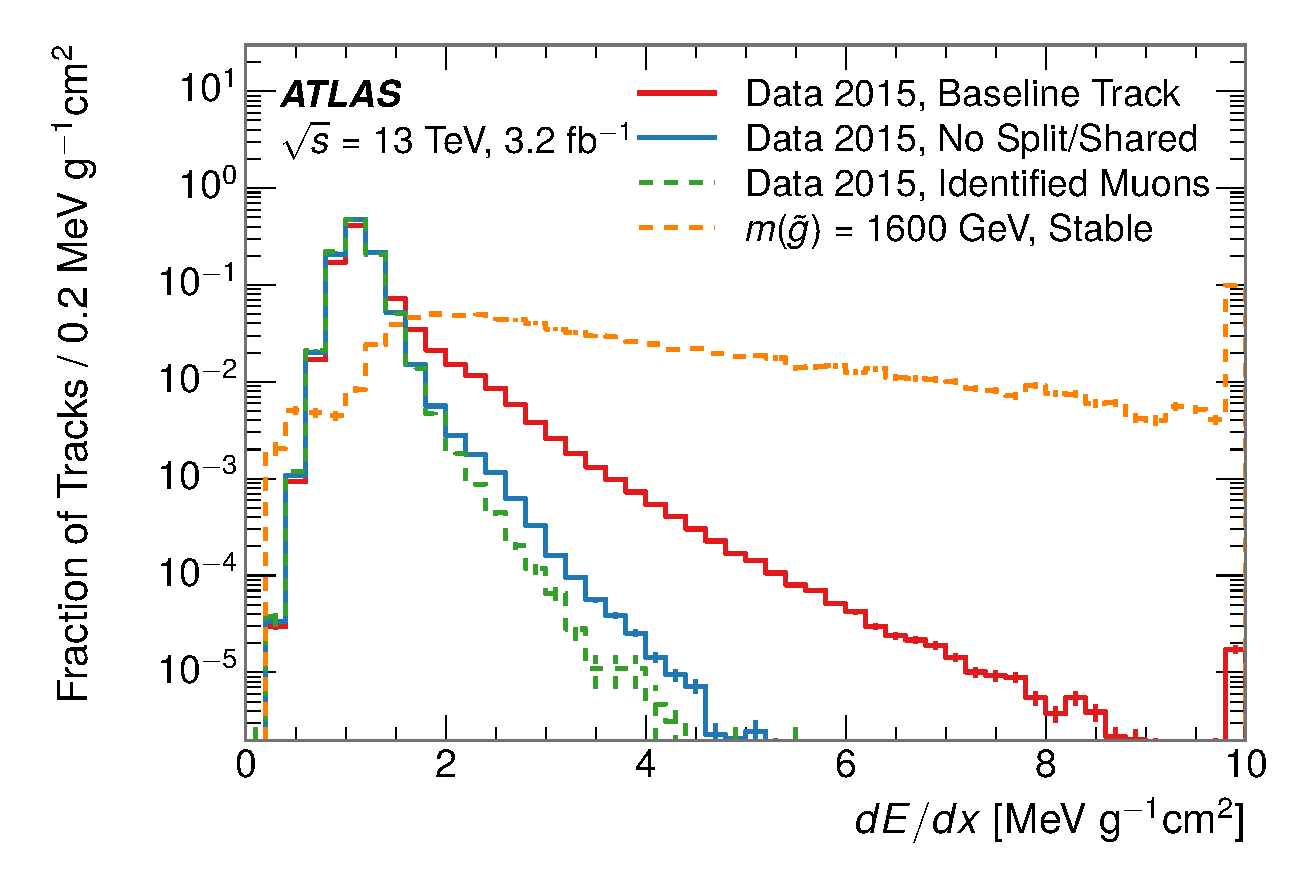
\includegraphics[width=\fullfig]{figures/dedx_isolation.pdf}
\caption{The distribution of \dedx with various selections applied in data and simulated signal events.}
\label{fig:dedx_isolation}
\end{figure}

A few additional kinematic requirements are imposed to help reduce \ac{SM} backgrounds. 
The momentum of the candidate track must be at least 150 \GeV, and the uncertainty on that measurement must be less than 50\%. 
The distribution of momentum is shown in Figure~\ref{fig:nm1_p} for tracks in data and simulated signal events after the previously discussed requirements on clusters, transverse momentum, and isolation have been imposed.
The signal particles are much harder on average than their backgrounds because of the high energy interactions required to produce them.
The transverse mass, \mt, defined as 

\begin{equation}
 \mt = \sqrt{2 \pt \met (1-\cos(\Delta\phi (\met,\mathrm{track})) ) }
\end{equation}

\noindent estimates the mass of a decay of to a single charged particle and an undetected particle and is required to be greater than 130 \GeV to reject contributions from the decay of W bosons.
Figure~\ref{fig:nm1_mt} shows the distribution of \mt for data and simulated signal events.
The signal is distributed over a wide range of \mt, with about 90\% above the threshold value of 130 \GeV. 
The data shows a dual-peaked structure, where the first peak comes from W boson decays and the second peak is a kinematic shaping from the requirements on \met and the track \pt in dijet events.

\begin{figure}[h]
\centering
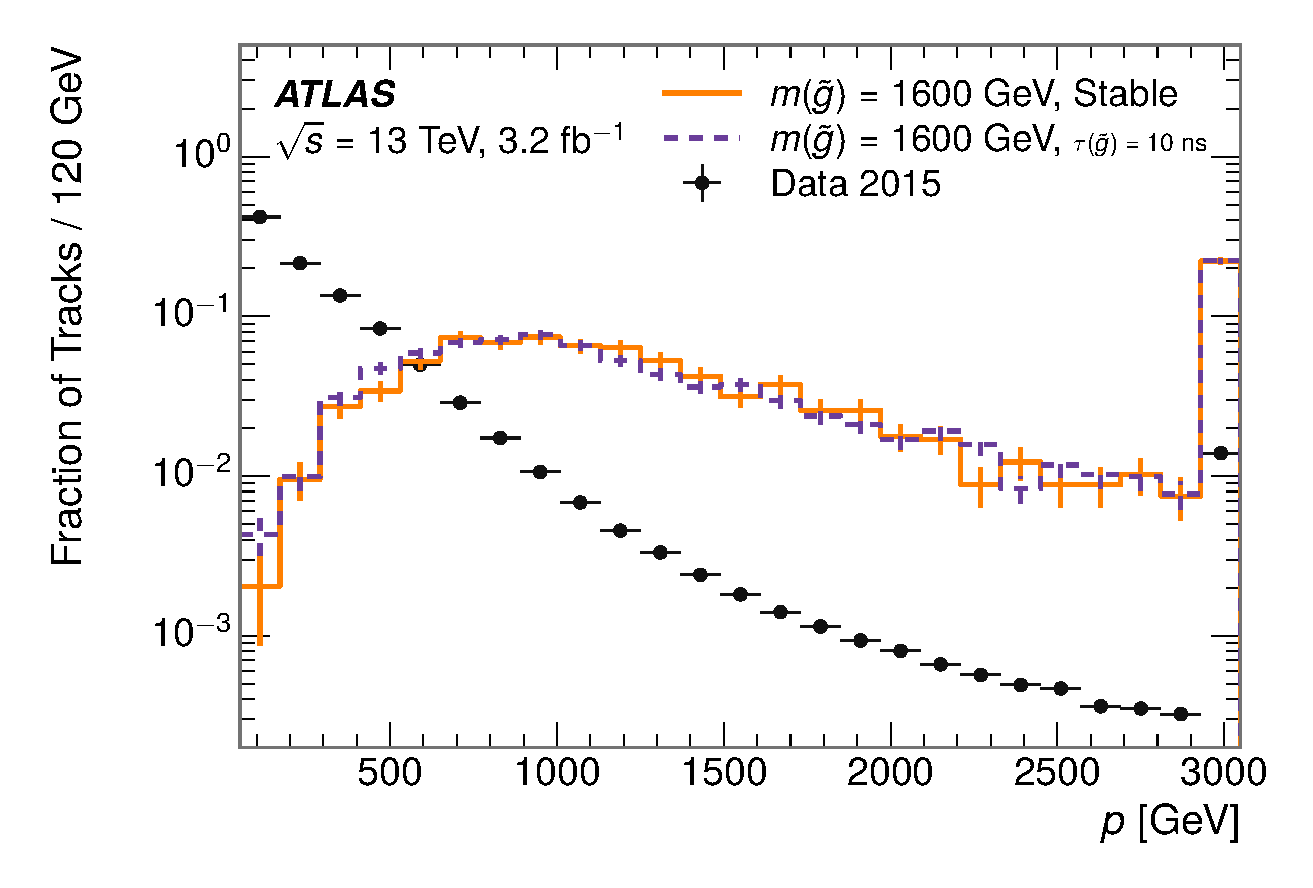
\includegraphics[width=\fullfig]{figures/selection_p_nm1.pdf}
\caption{The distribution of track momentum for data and simulated signal events, after previous selection requirements have been applied.}
\label{fig:nm1_p}
\end{figure}


\begin{figure}[h]
\centering
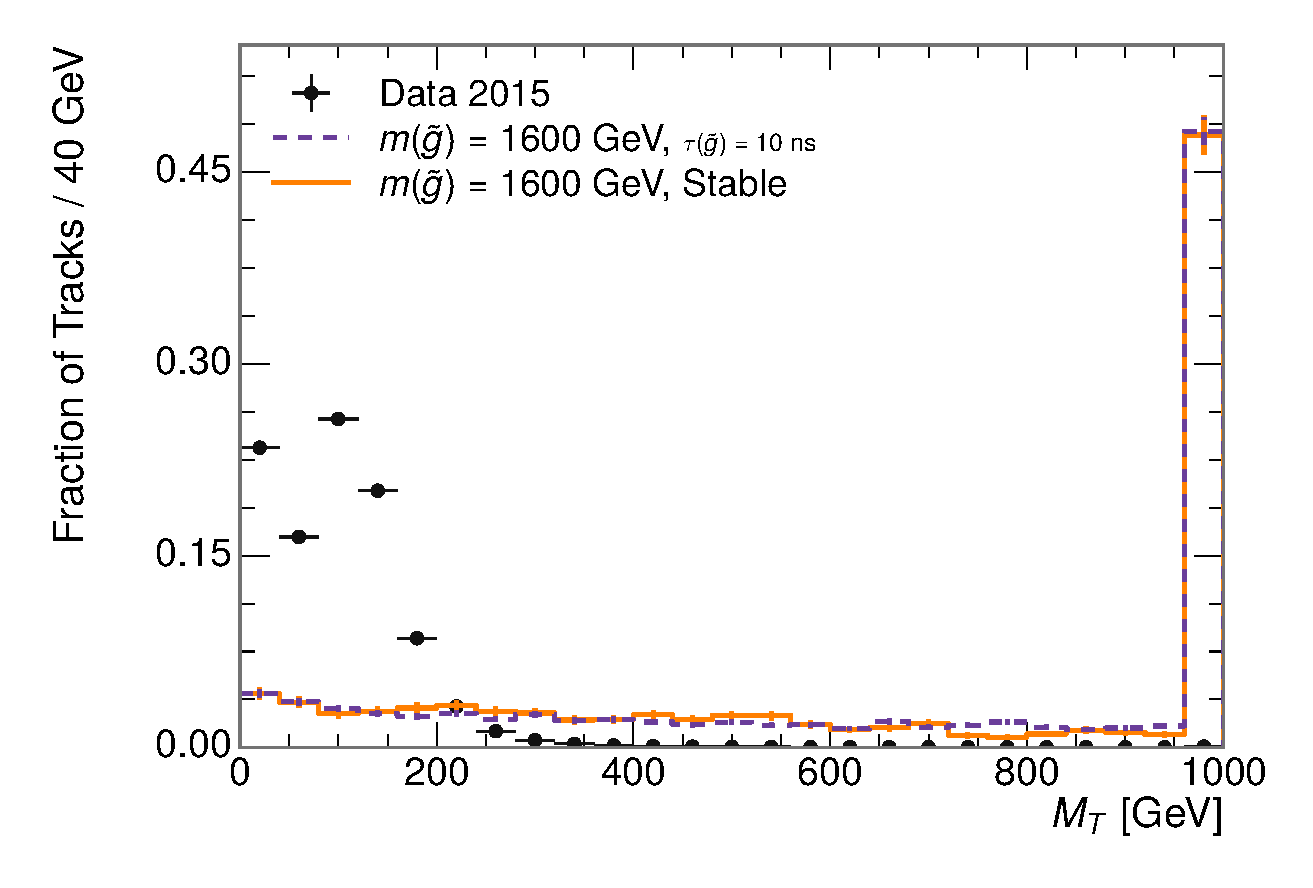
\includegraphics[width=\fullfig]{figures/selection_mt_nm1.pdf}
\caption{The distribution of $M_T$ for data and simulated signal events, after previous selection requirements have been applied.}
\label{fig:nm1_mt}
\end{figure}

% ----------------------------------------

\section{Particle Species Rejection}
\label{sec:sm_rejection}

The amount of ionization deposited by particles with low mass and high momentum has a large positive tail~\cite{pdg}, so backgrounds can be formed by a wide variety of \ac{SM} processes when various charged particles have a few randomly large deposits of energy in the pixel detector.
Those backgrounds can be additionally reduced by targeting other interactions with the detector where they are expected to have different behavior than \rhadrons.
The interactions with the detector depend on the types of particles produced rather than the processes which produce them, so this search forms a series of rejections to remove backgrounds from individual particle species.
These rejections focus on using additional features of the event, other than the kinematics of the candidate track, as they can provide a powerful source of background rejection with very high signal efficiency.
However, the lifetime of an \rhadron can significantly change its detector characteristics, as discussed in Section~\ref{sec:rh_lifetimes}.
To accommodate these differences, the \ac{SM} rejections defined in this section are split to form two signal regions, one for long-lifetimes particles, the stable region ($50 <= \tau [\mathrm{ns}] < \inf$ ns), and one for intermediate lifetime particles, the metastable region ($0.4 < \tau [\mathrm{ns}] < 50$).

Jets can be very effectively rejected by considering the larger-scale isolation of the candidate track.
In this case the isolation focuses on the production of nearby particles as a jet-veto, rather than the isolation from overlapping tracks based on \Nsplit that was used to reduce high-ionization backgrounds.
As explained in Section~\ref{sec:characteristics}, the fragmentation process which produces an \rhadron is very hard and thus is not expected to produce additional particles with a summed momentum of more than 5 \GeV.
The jet-veto uses the summed momentum of tracks with a cone of $\Delta R < 0.25$, referred to as \ptcone, which is shown in Figure~\ref{fig:nm1_isopt} for data and simulated signal events. 
In the data this value has a peak at zero from isolated tracks such as leptons, and a long tail from jets which contains as much as 80\% of the background above 20 \GeV at this stage of the selection.
In signal events \ptcone is strongly peaked at zero and significantly less than 1\%  of signal events have \ptcone above 20 \GeV. 
This makes a requirement of $\ptcone < 20$ \GeV a very effective method to reject background without losing signal efficiency.
For the stable signal region, this cut is further tightened to $\ptcone < 5$ \GeV as it is the most effective variable remaining to extend the search reach for long lifetimes.

\begin{figure}[h]
\centering
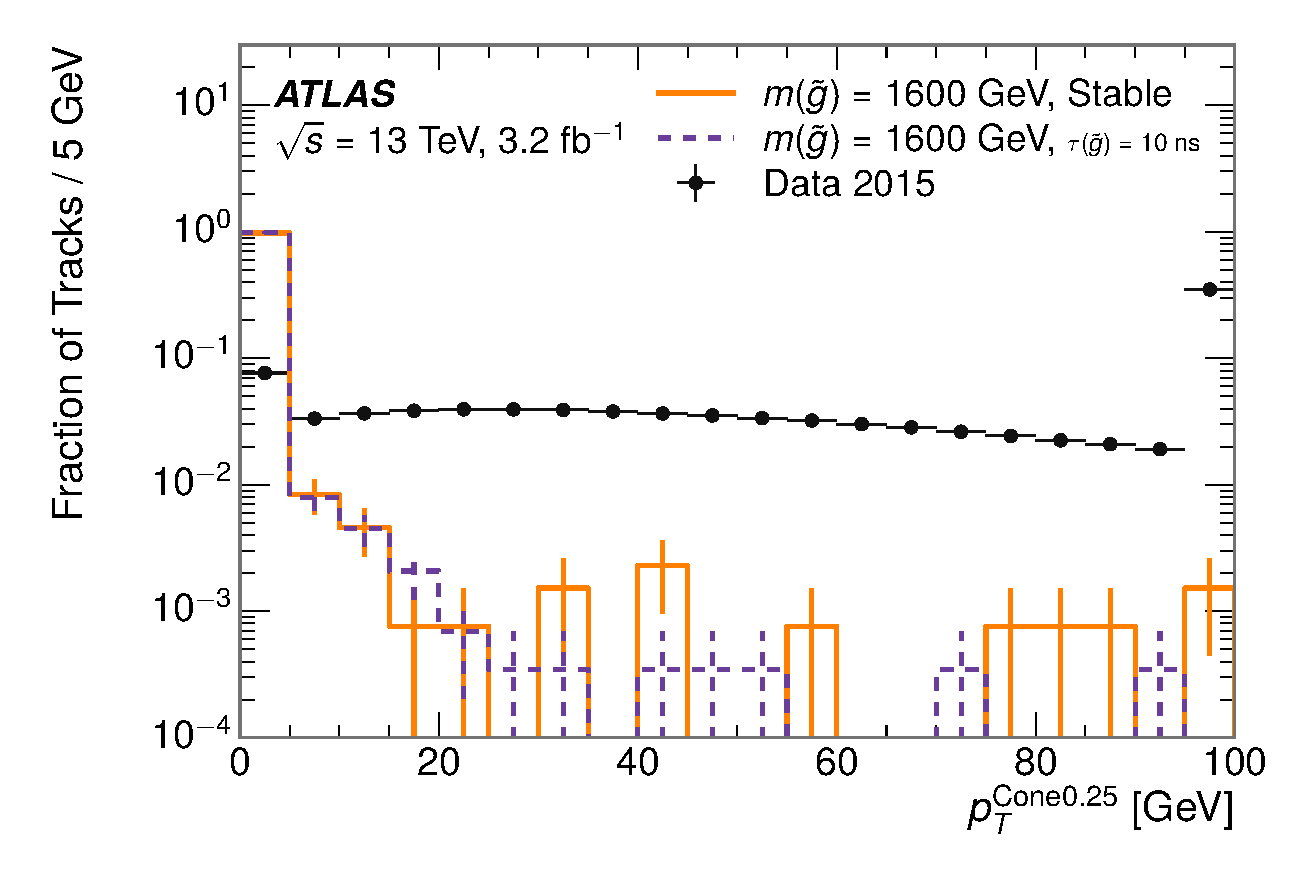
\includegraphics[width=\fullfig]{figures/selection_isopt_nm1.pdf}
\caption{The distribution of summed tracked momentum within a cone of $\Delta R < 0.25$ around the candidate track for data and simulated signal events, after previous selection requirements have been applied.}
\label{fig:nm1_isopt}
\end{figure}

Even for fully isolated particles, there are additional methods to reject each type of particle using information in the muon system and calorimeters.
Muons can be identified very reliably using the tracks in the muon system, as described in Section~\ref{sec:muons}.
For intermediate lifetimes the \acp{LLP} do not survive long enough to reach the muon system, and so muons are vetoed by rejecting tracks that associate to a muon with medium muon identification requirements (Section~\ref{sec:muons}).
For longer lifetimes, this rejection is not applied because \acp{LLP} which reach the muon system can be identified as muons as often as 30\% of the time in simulated samples.

Calorimeter-based particle rejection relies on the expected small deposits of energy from \acp{LLP}. 
When the lifetime is long enough to reach the calorimeter, a \ac{LLP} deposits little of its energy as it traverses the material, as discussed in Section~\ref{sec:characteristics}. 
Even when the particle does decay before the calorimeter, the majority of its energy is carried away by the \ac{LSP} and not deposited in the calorimeter.
In both cases the energy is expected to be distributed across the layers of the calorimeters and not peaked in just one layer. 
This can be quantified in terms of \ep, the ratio of calorimeter energy of a nearby jet to the track momentum, and \emfrac, the fraction of energy in that jet within the electromagnetic calorimeter.
When no jets fall within a cone of 0.05 of the particle, \ep and \emfrac are both defined as zero.
\ep is expected to be above 1.0 for typical \ac{SM} particles because of calibration and the contributions from other nearby particles, as discussed in Chapter~\ref{ch:singlehadrons}.
At these momenta there is no significant zero fraction due to interactions with the detector or insufficient energy deposits (see Section~\ref{sec:zero_fraction}). 
\emfrac is peaked close to 1.0 for electrons, and distributed between 10\% and 90\% for hadrons.

These trends can be seen in the two dimensional distribution for signal in Figure~\ref{fig:eoverp_emfrac} for stable and metastable (10 ns) events.
The majority of \rhadrons in both samples fall into the bin for $\ep = 0$ and $\emfrac = 0$ because the majority of the time there is no associated jet. 
In the stable sample, when there often is an associated jet, \ep is typically still below 0.1, and the \emfrac is predominantly under 0.8.
In the metastable sample, on the other hand, \ep is larger but still typically below 0.1 because of actual jets produced during the decay.
The \emfrac is much lower on average in this case, below 0.1, because the 10 ns lifetime particles rarely decay before passing through the electromagnetic calorimeter.
Figure~\ref{fig:eoverp_emfrac} also includes simulated Z decays to electrons or tau leptons.
From the decays to electrons it is clear that the majority of electrons have \emfrac above 0.9.
The tau decays include a variety of products.
Muons can be seen in the bin where $\ep = 0$ and $\emfrac = 0$ because they do not have an associated jet.
Electrons fall into the range where $\ep > 1$ and $\emfrac > 0.9$.
Hadronic tau decays are the most common, and fall in the range of $0.1 < \emfrac < 0.9$ and $\ep > 1.0$. 

\begin{figure}[htb]
\centering
\subfloat[]{
  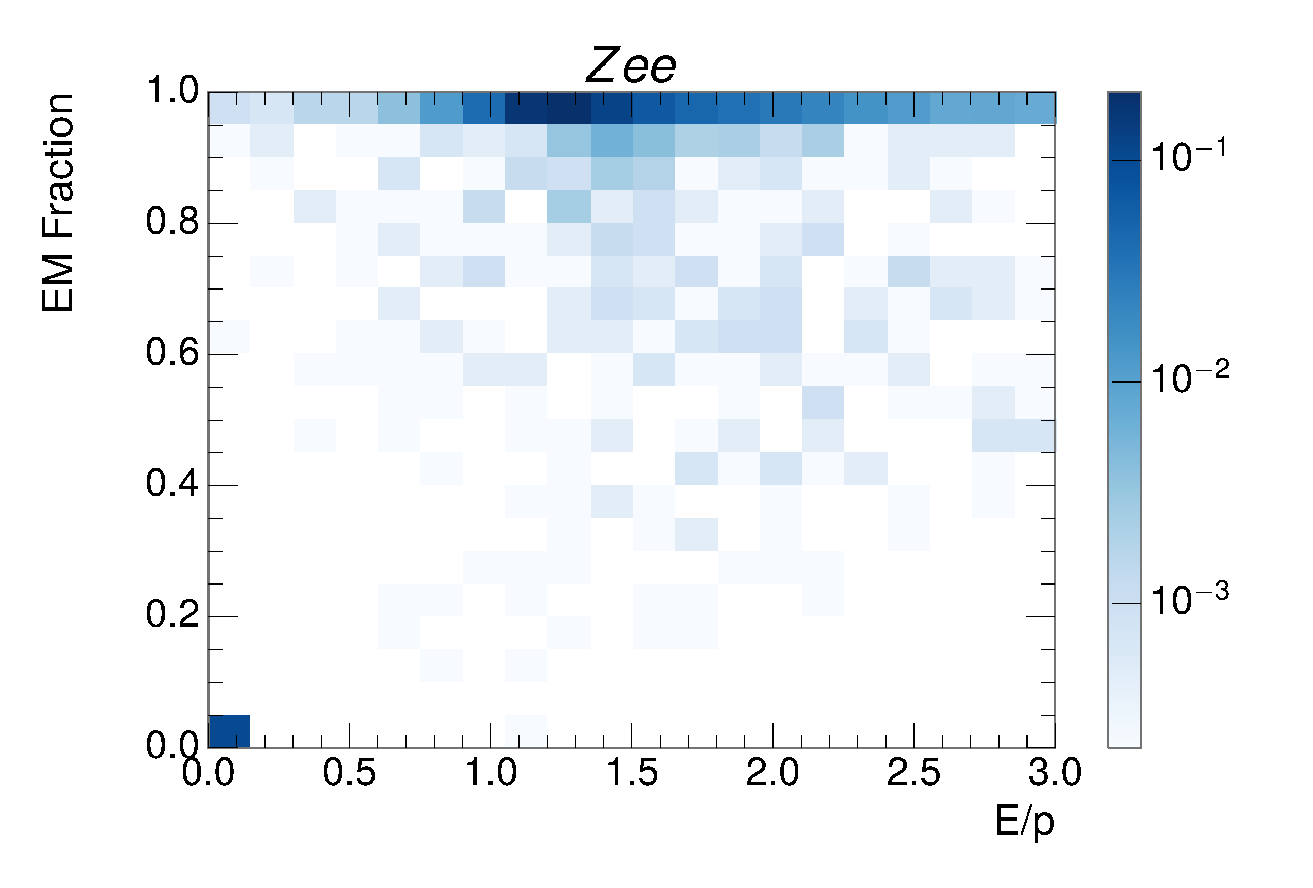
\includegraphics[width=\halffig]{figures/zee_eoverp_emfrac.pdf}
}
\subfloat[]{
  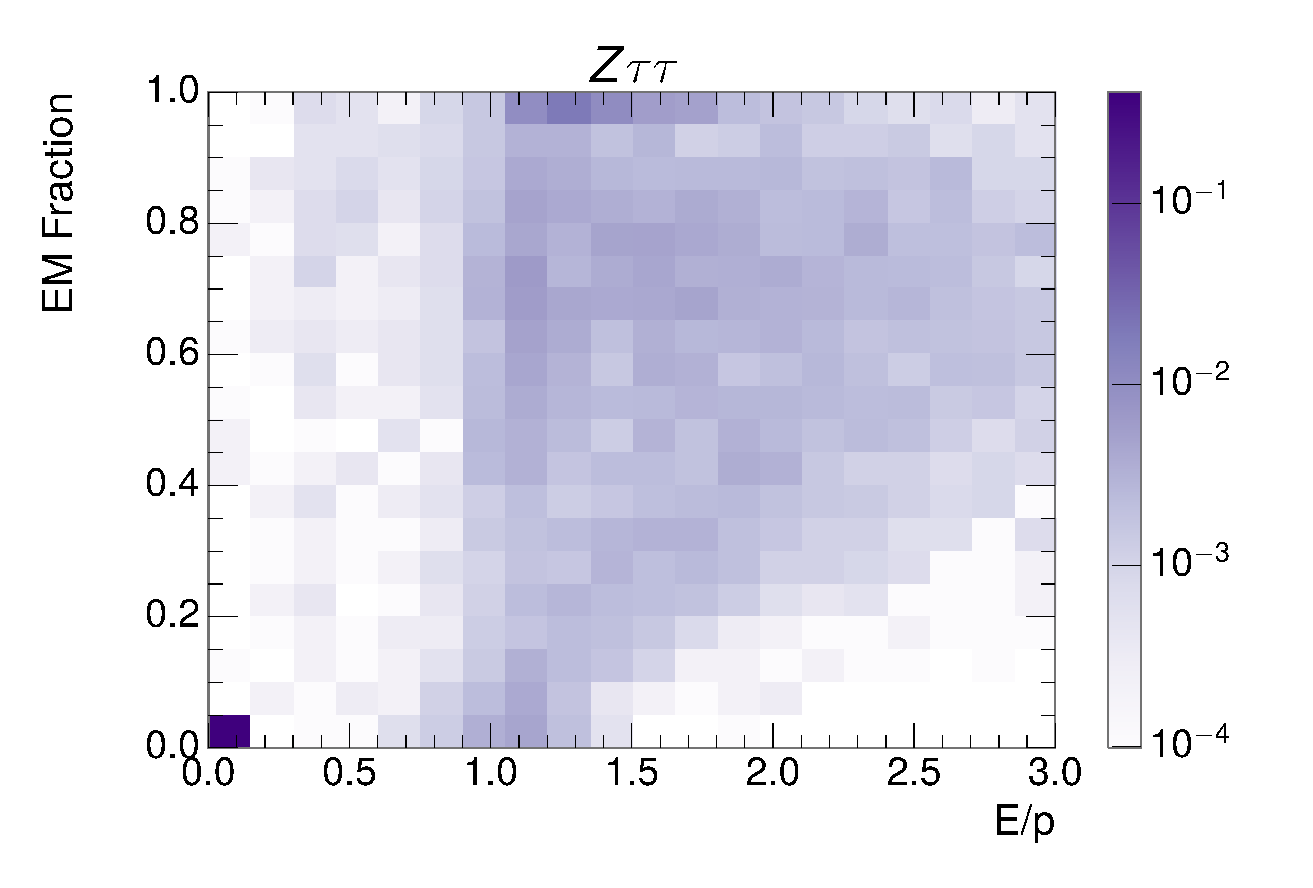
\includegraphics[width=\halffig]{figures/ztautau_eoverp_emfrac.pdf}
}\\
\subfloat[]{
  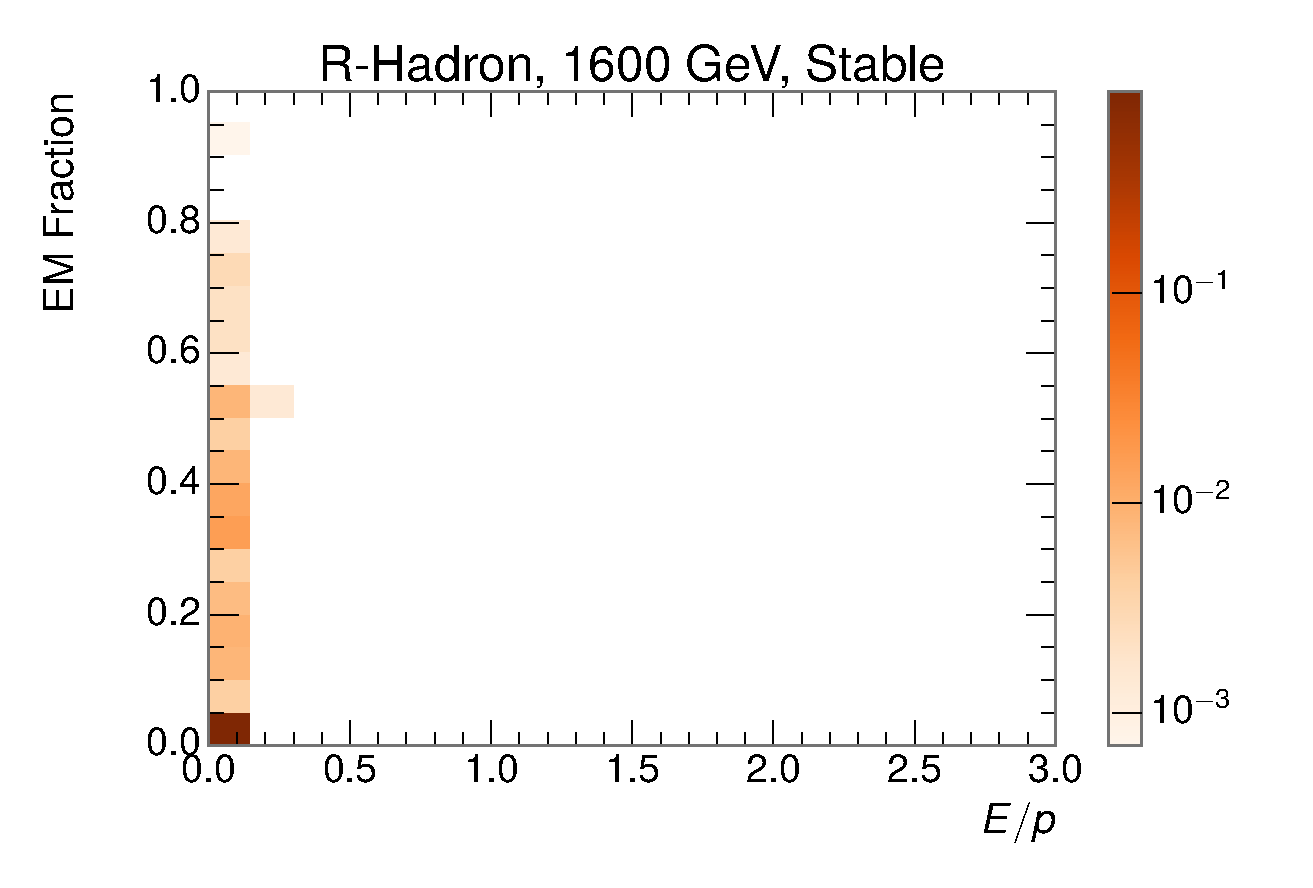
\includegraphics[width=\halffig]{figures/stable_eoverp_emfrac.pdf}
}
\subfloat[]{
  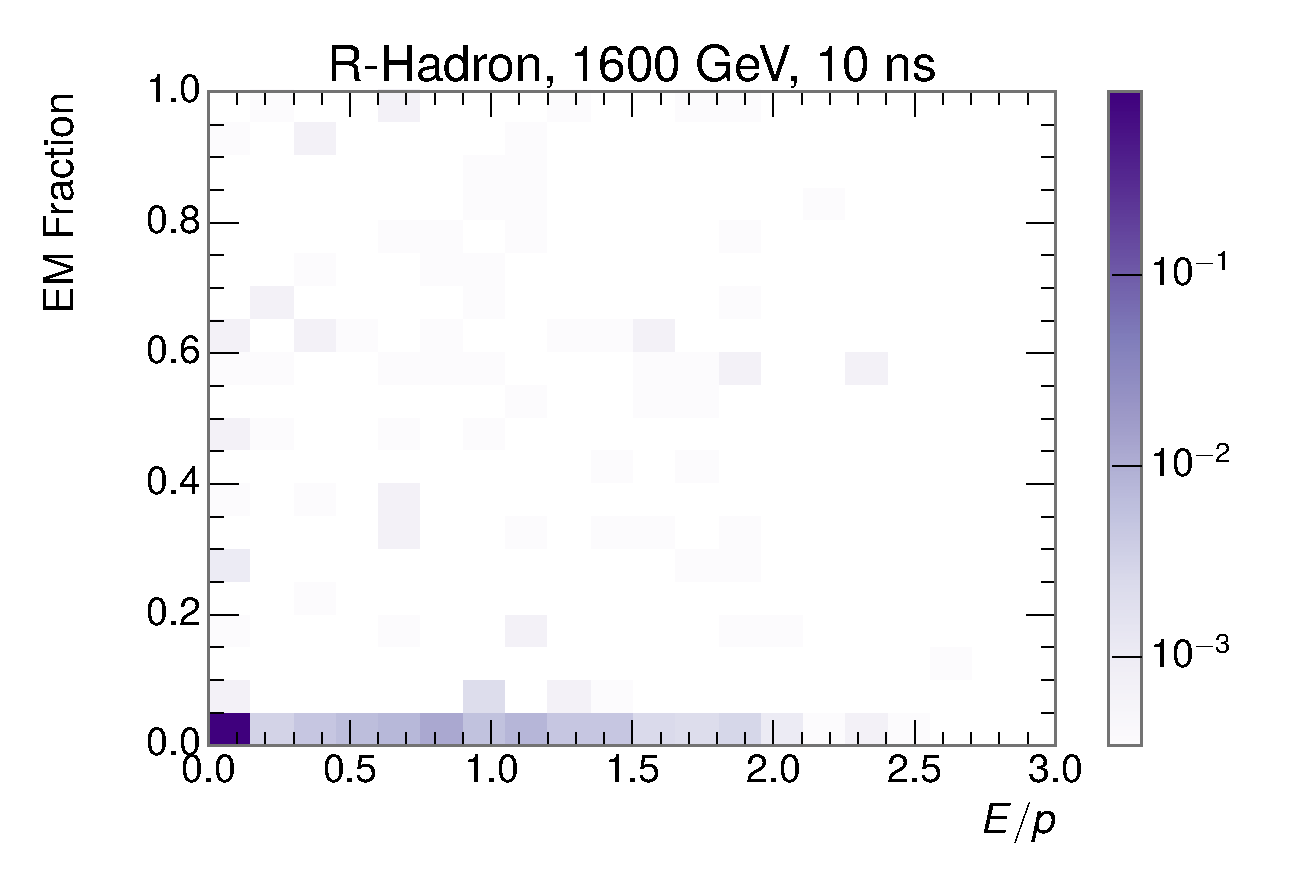
\includegraphics[width=\halffig]{figures/metastable_eoverp_emfrac.pdf}
}
\caption{The normalized, two-dimensional distribution of $E/p$ and \emfrac for simulated (a) $Z\rightarrow e e$, (b) $Z\rightarrow \tau\tau$, (c) 1200 \GeV Stable R-Hadron events, and (d) 1200 \GeV, 10 ns R-Hadron events.}
\label{fig:eoverp_emfrac}
\end{figure}

These differences motivate an electron rejection by requiring an \emfrac below 0.9.
Similarly, isolated hadrons are rejected by requiring $\ep < 1.0$.
These requirements combine to remove the majority of isolated electrons and hadrons but retain over 95\% of the simulated signal across a range of masses and lifetimes.

% ----------------------------------------

\section{Ionization}

The final requirement on the candidate track is the primary discriminating variable, the ionization in the pixel detector.
That ionization is measured in terms of \dedx, which was shown for data and simulated signal events in Figure~\ref{fig:dedx_isolation}.
\dedx is dramatically greater for the high mass signal particles than the backgrounds, which start to fall immediately after the minimally ionizing peak at 1.1 \MeVgcm. 
The \dedx for candidate tracks must be greater than a pseudorapidity-dependent threshold, specifically $1.80 - 0.11 |\eta| + 0.17 \eta^2 - 0.05 |\eta|^3 $~\MeV~g$^{-1}$~cm$^{-2}$, in order to correct for an approximately 5\% dependence of the \ac{MIP} peak on $\eta$. 
The requirement was chosen as part of the signal region optimization, and manages to reduce the backgrounds by a factor of 100 while remaining 70-90\% efficient for simulated signal events depending on the mass.

\subsection{Mass Estimation}
\label{sec:mass_requirement}
The mean value of ionization in silicon is governed by the Bethe equation and the most probable value follows a Landau-Vavilov distribution~\cite{pdg}. 
Those forms inspire a parametric description of \dedx in terms of $\beta\gamma$, 

\begin{equation}
(\dedx)_\mathrm{MPV}(\beta \gamma) = {p_1\over \beta^{p_3}}\ln(1+[p_2\beta\gamma]^{p_5})-p_4 \label{eq:bbfun}
\end{equation}

\noindent which performs well in the range $0.3< \beta\gamma<1.5$.
This range includes the expected range of $\beta\gamma$ for the particles targeted for this search, with $\beta\gamma \approx 2.0$ for lower mass particles (O(100 \GeV)) and up to $\beta\gamma \approx 0.5$ for higher mass particles (O(1000 \GeV)). 
The parameters, $p_i$, are fit using a 2015 data sample of low-momentum pions, kaons, and protons as described in Ref.~\cite{dedxnote}. 
Figure~\ref{fig:dedx_momentum} shows the two-dimensional distribution of \dedx and momentum along with the above fitted values for $(\dedx)_\mathrm{MPV}$.

\begin{figure}
\centering
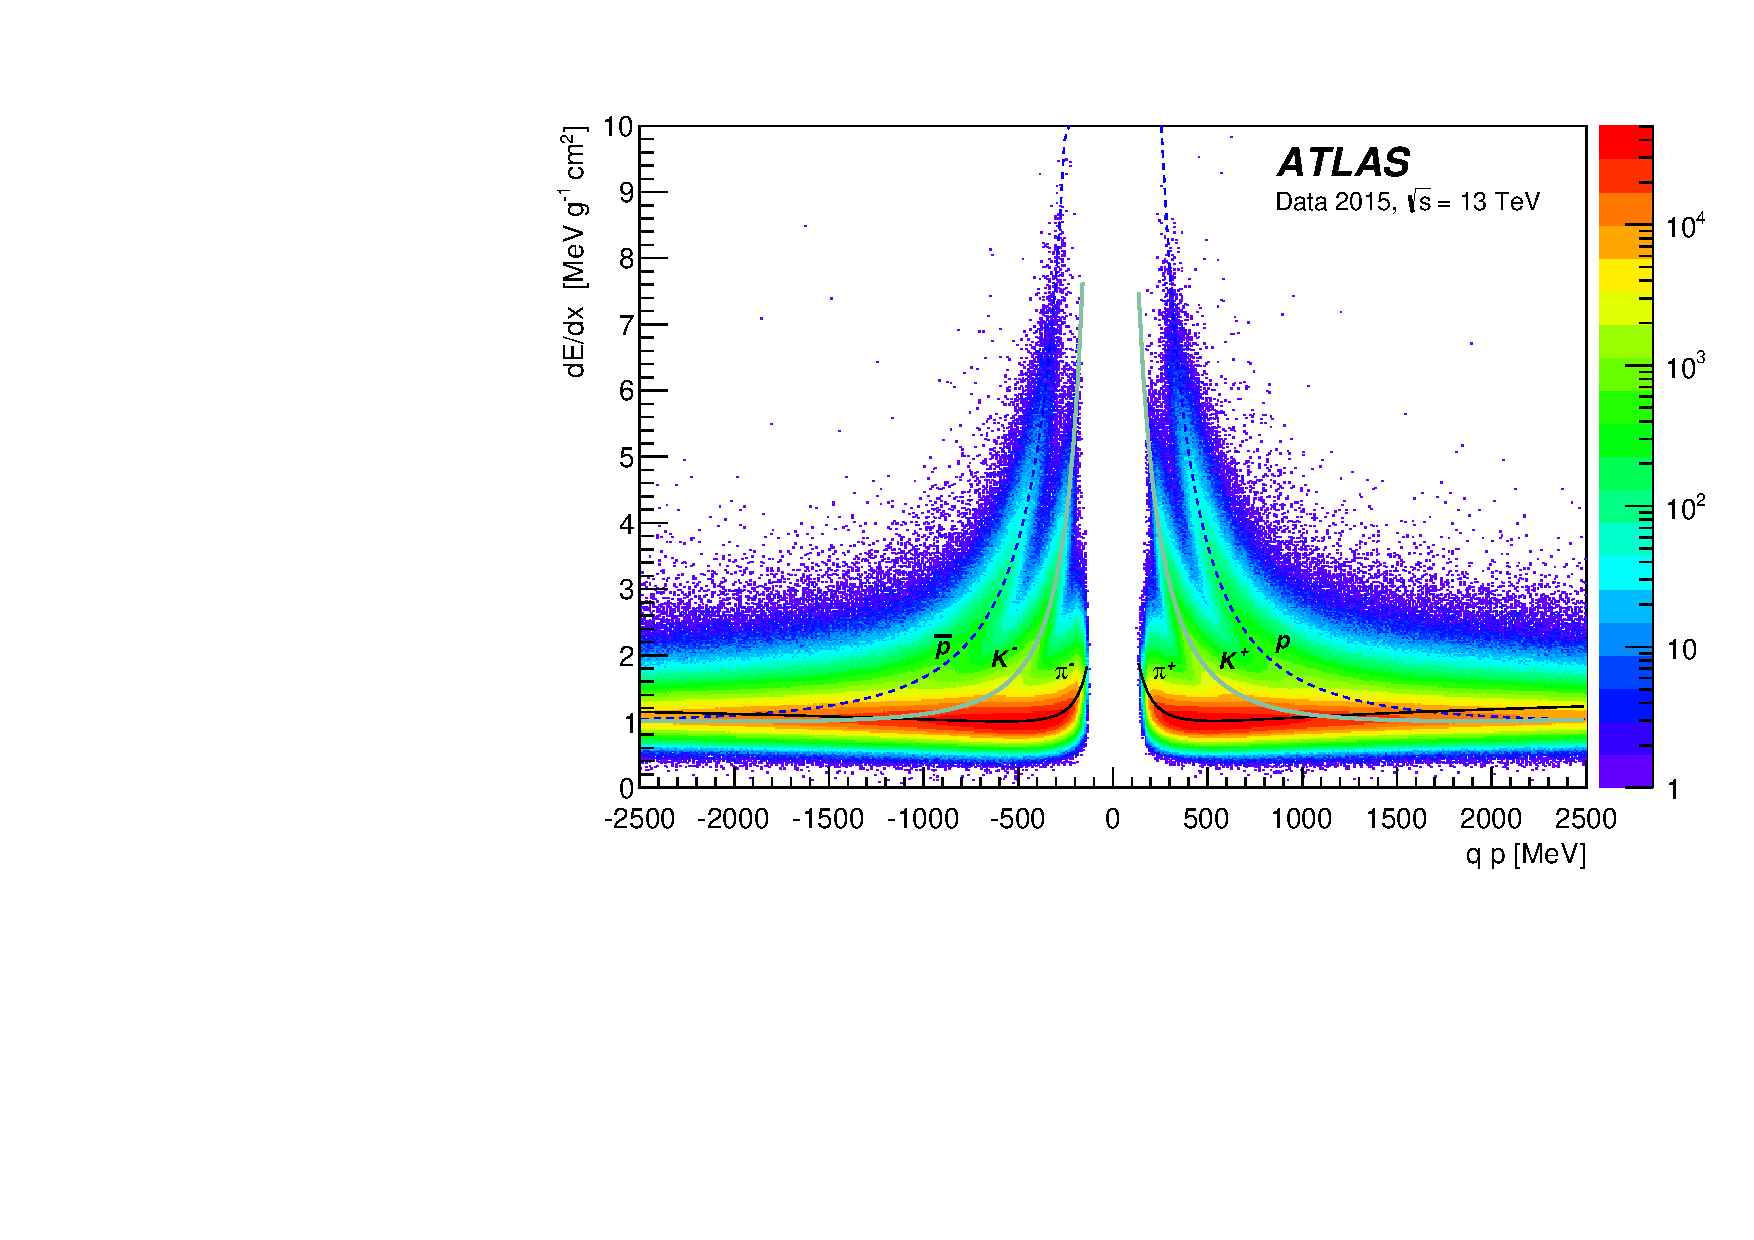
\includegraphics[width=\fullfig]{figures/dedx_momentum.pdf}
\caption{Two-dimensional distribution of $\dedx$ versus charge signed momentum (qp) for minimum-bias tracks. The fitted distributions of the most probable values for pions, kaons and protons are superimposed.}
\label{fig:dedx_momentum}
\end{figure}

The above equation~(\ref{eq:bbfun}) is then numerically inverted to estimate $\beta\gamma$ and the mass for each candidate track.
In simulated signal events, the mean of this mass value reproduces the generated mass up to around 1800 \GeV to within 3\%, and 3\% shift is applied to correct for this difference.
The mass distributions prior to this correction are shown for a few stable mass points in Figure~\ref{fig:mass_dedx}.
The large widths of these distributions come from the high variability in energy deposits in the pixel detector as well as the uncertainty on momentum measurements at high momentum, but the means converge to the expected values.

\begin{figure}
\centering
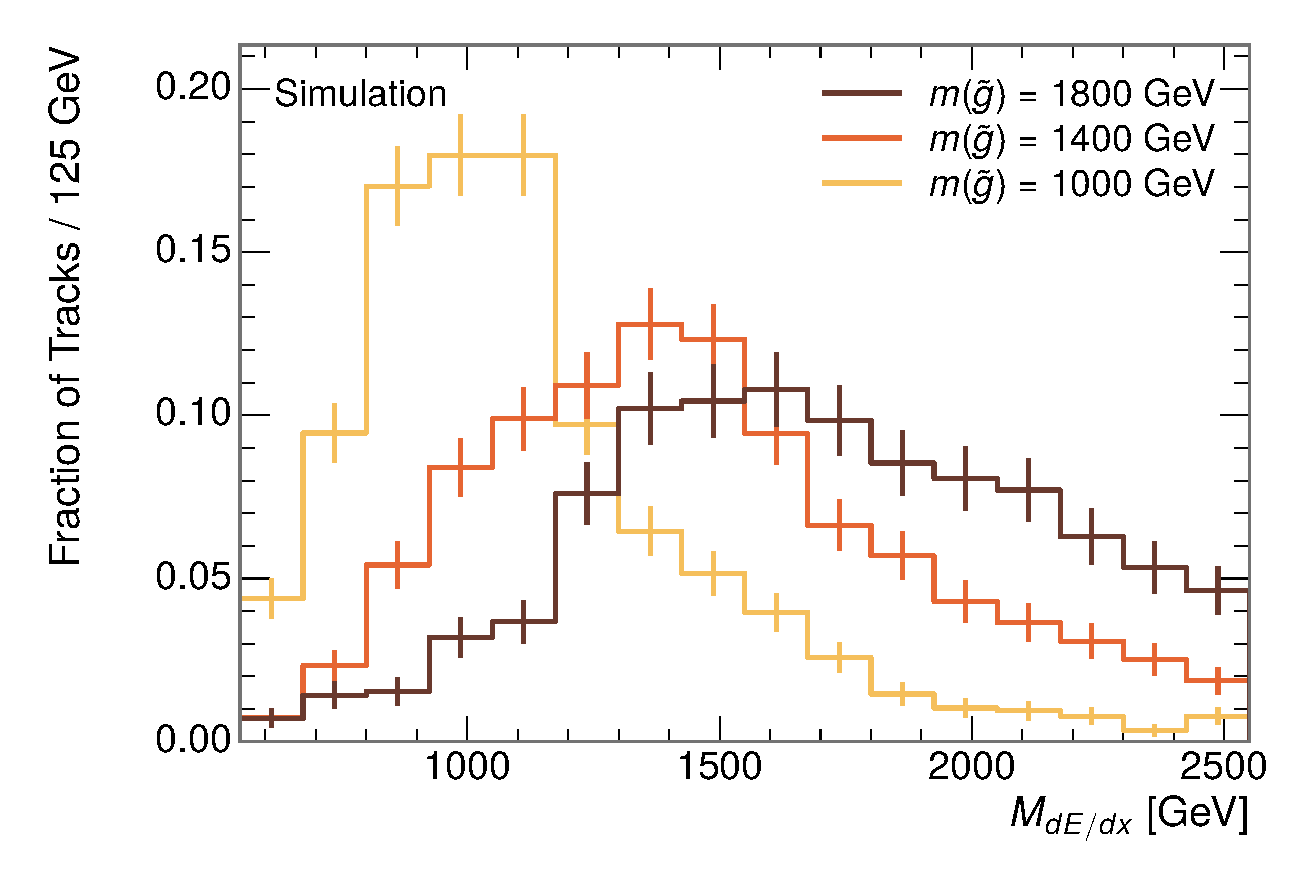
\includegraphics[width=\fullfig]{figures/mass_dedx.pdf}
\caption{The distribution of mass estimated using \dedx for simulated stable \rhadrons with masses between 1000 and 1600 \GeV.}
\label{fig:mass_dedx}
\end{figure}

This analysis evaluates expected yields and the resulting cross sectional limits using windows in this mass variable.
The windows are formed by fitting mass distributions in simulated signal events like those in Figure~\ref{fig:mass_dedx} to Gaussian distributions and taking all events that fall within $\pm 1.4 \sigma$ of the mean.
As can be seen in Figure~\ref{fig:mass_dedx}, typical values for this width are $\sigma \approx 300-500$ \GeV depending on the generated mass.

\section{Efficiency}
\label{sec:efficiency}

The numbers of events passing each requirement through ionization are shown in Table~\ref{tab:cutflow} for the full 2015 dataset and a simulated 1600 \GeV, 10 ns lifetime \rhadron sample. 
The table highlights the overall acceptance $\times$ efficiency for signal events, which for this example is 19\%.
Between \ac{SM} rejection and ionization, this signal region reduces the background of tracks which pass the kinematic requirements down by an additional factor of almost 2000.

\begin{table}[h]
\centering
\begin{tabular}{l r r}
  \hline
  Selection & Exp. Signal Events & Observed Events in \lumi~fb\tsup{-1} \\
  \hline
  Generated                    & 26.0 $\pm$ 0.3          & \\
  \met Trigger                 & 24.8 $\pm$ 0.3 ($95\%$) & \\
  $\met > 130$ \GeV            & 23.9 $\pm$ 0.3 ($92\%$) & \\
  Track Quality and $\pt > 50$ & 10.7 $\pm$ 0.2 ($41\%$) & 368324 \\
  Isolation Requirement        & 9.0  $\pm$ 0.2 ($35\%$) & 108079 \\
  Track $p > 150$ \GeV         & 6.6  $\pm$ 0.2 ($25\%$) & 47463 \\
  $\mt > 130$ \GeV             & 5.8  $\pm$ 0.2 ($22\%$) & 18746 \\
  Electron and Hadron Veto     & 5.5  $\pm$ 0.2 ($21\%$) & 3612 \\
  Muon Veto                    & 5.5  $\pm$ 0.2 ($21\%$) & 1668 \\
  Ionization Requirement       & 5.0  $\pm$ 0.1 ($19\%$) & 11 \\
  \hline
\end{tabular}
\caption{The expected number of events at each level of the selection for metastable 1600~\GeV, 10 ns \rhadrons, along with the number of events observed in data, for \lumi~fb\tsup{-1}. The simulated yields are shown with statistical uncertainties only. The total efficiency $\times$ acceptance is also shown for the signal.}
\label{tab:cutflow}
\end{table}


There is a strong dependence of this efficiency on lifetime and mass, with efficiencies dropping to under 1\% at low lifetimes.
Figure~\ref{fig:efficiency} shows the dependence on both mass and lifetime for all signal samples considered in this search.
The dependence on mass is relatively slight and comes predominantly from the increasing fraction of \rhadrons which pass the ionization cut with increasing mass.
The trigger and \met requirements are most efficient for particles that decay before reaching the calorimeters.
However, the chance of a particle to be reconstructed as a high-quality track decreases significantly at low lifetimes as the particle does not propagate sufficiently through the inner detector.
These effects lead to a maximum in the selection efficiency for lifetimes around 10-30 ns.

\begin{figure}
\centering
\subfloat[]{
  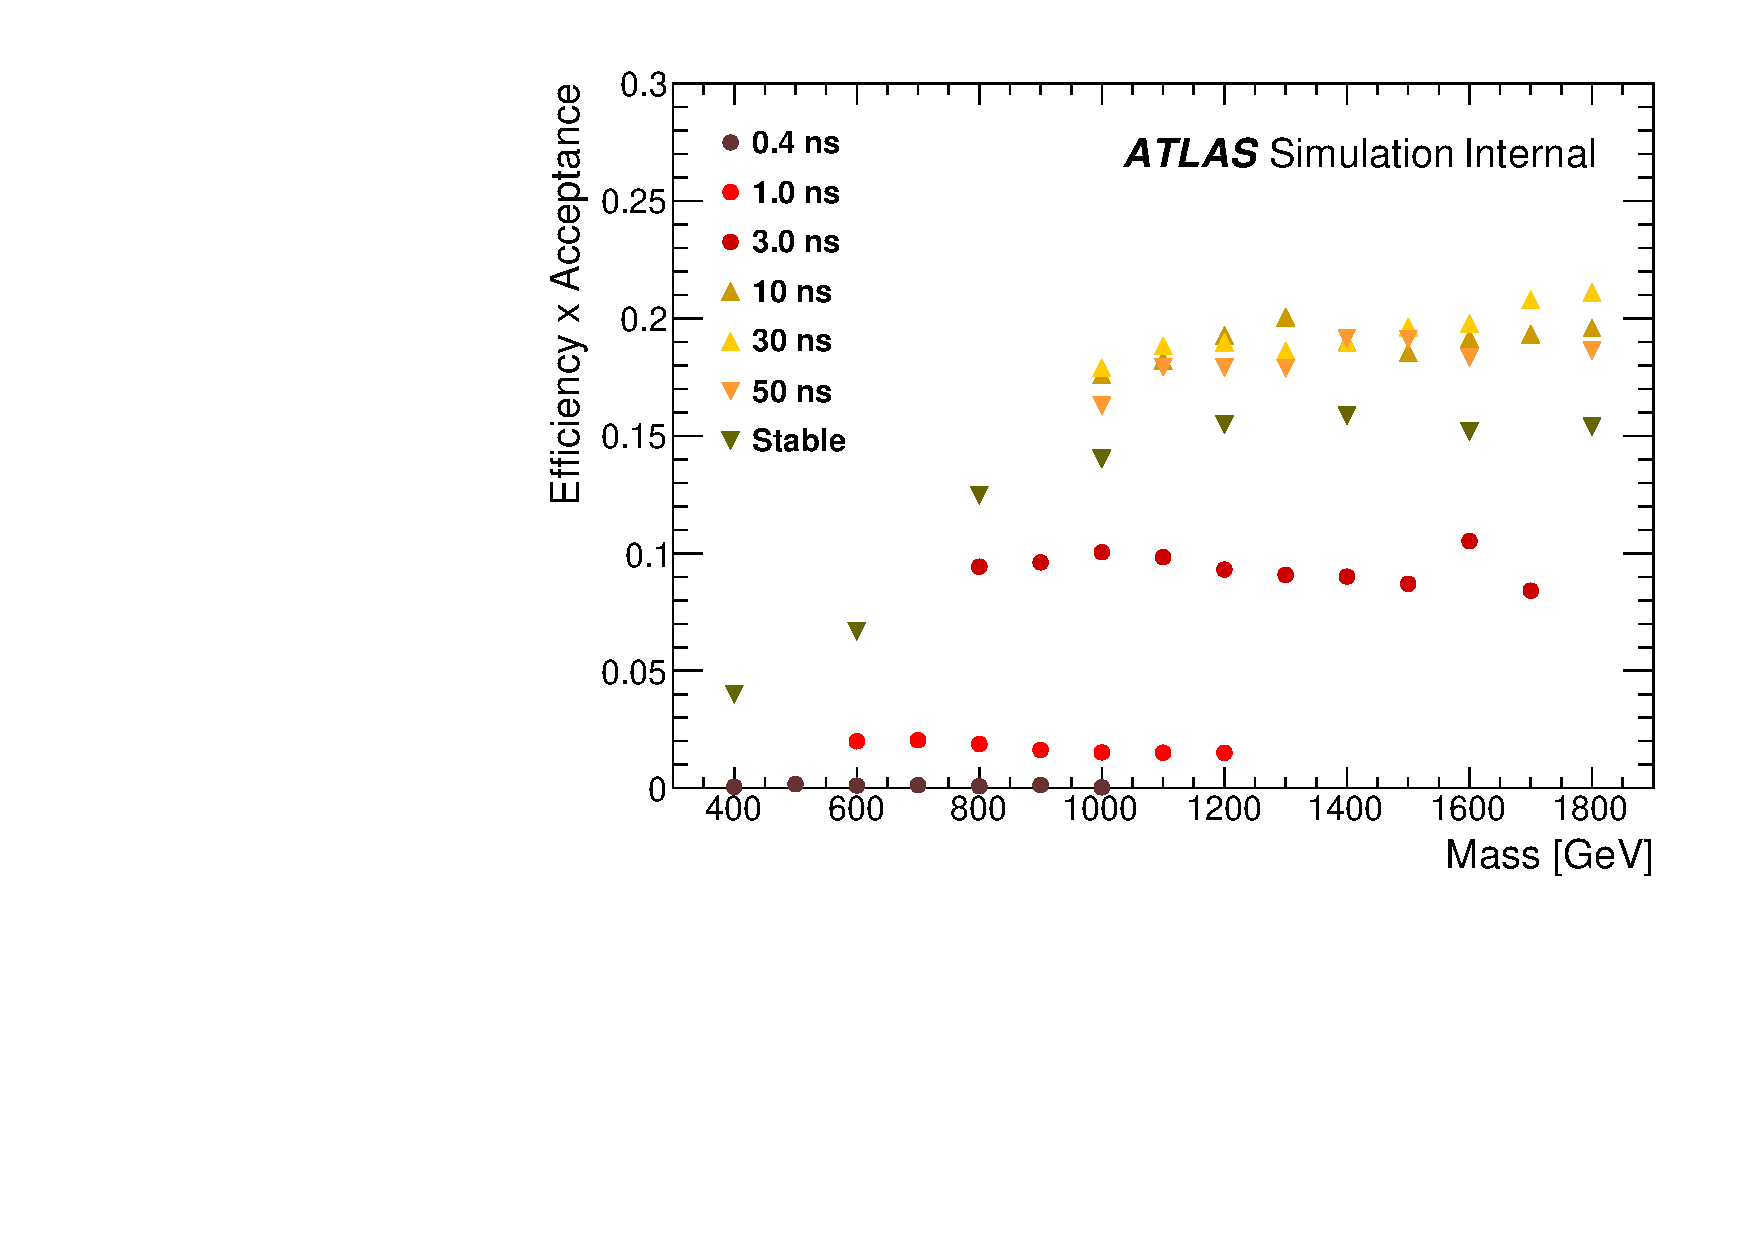
\includegraphics[width=\halffig]{figures/efficiency_mass.pdf}
}
\subfloat[]{
  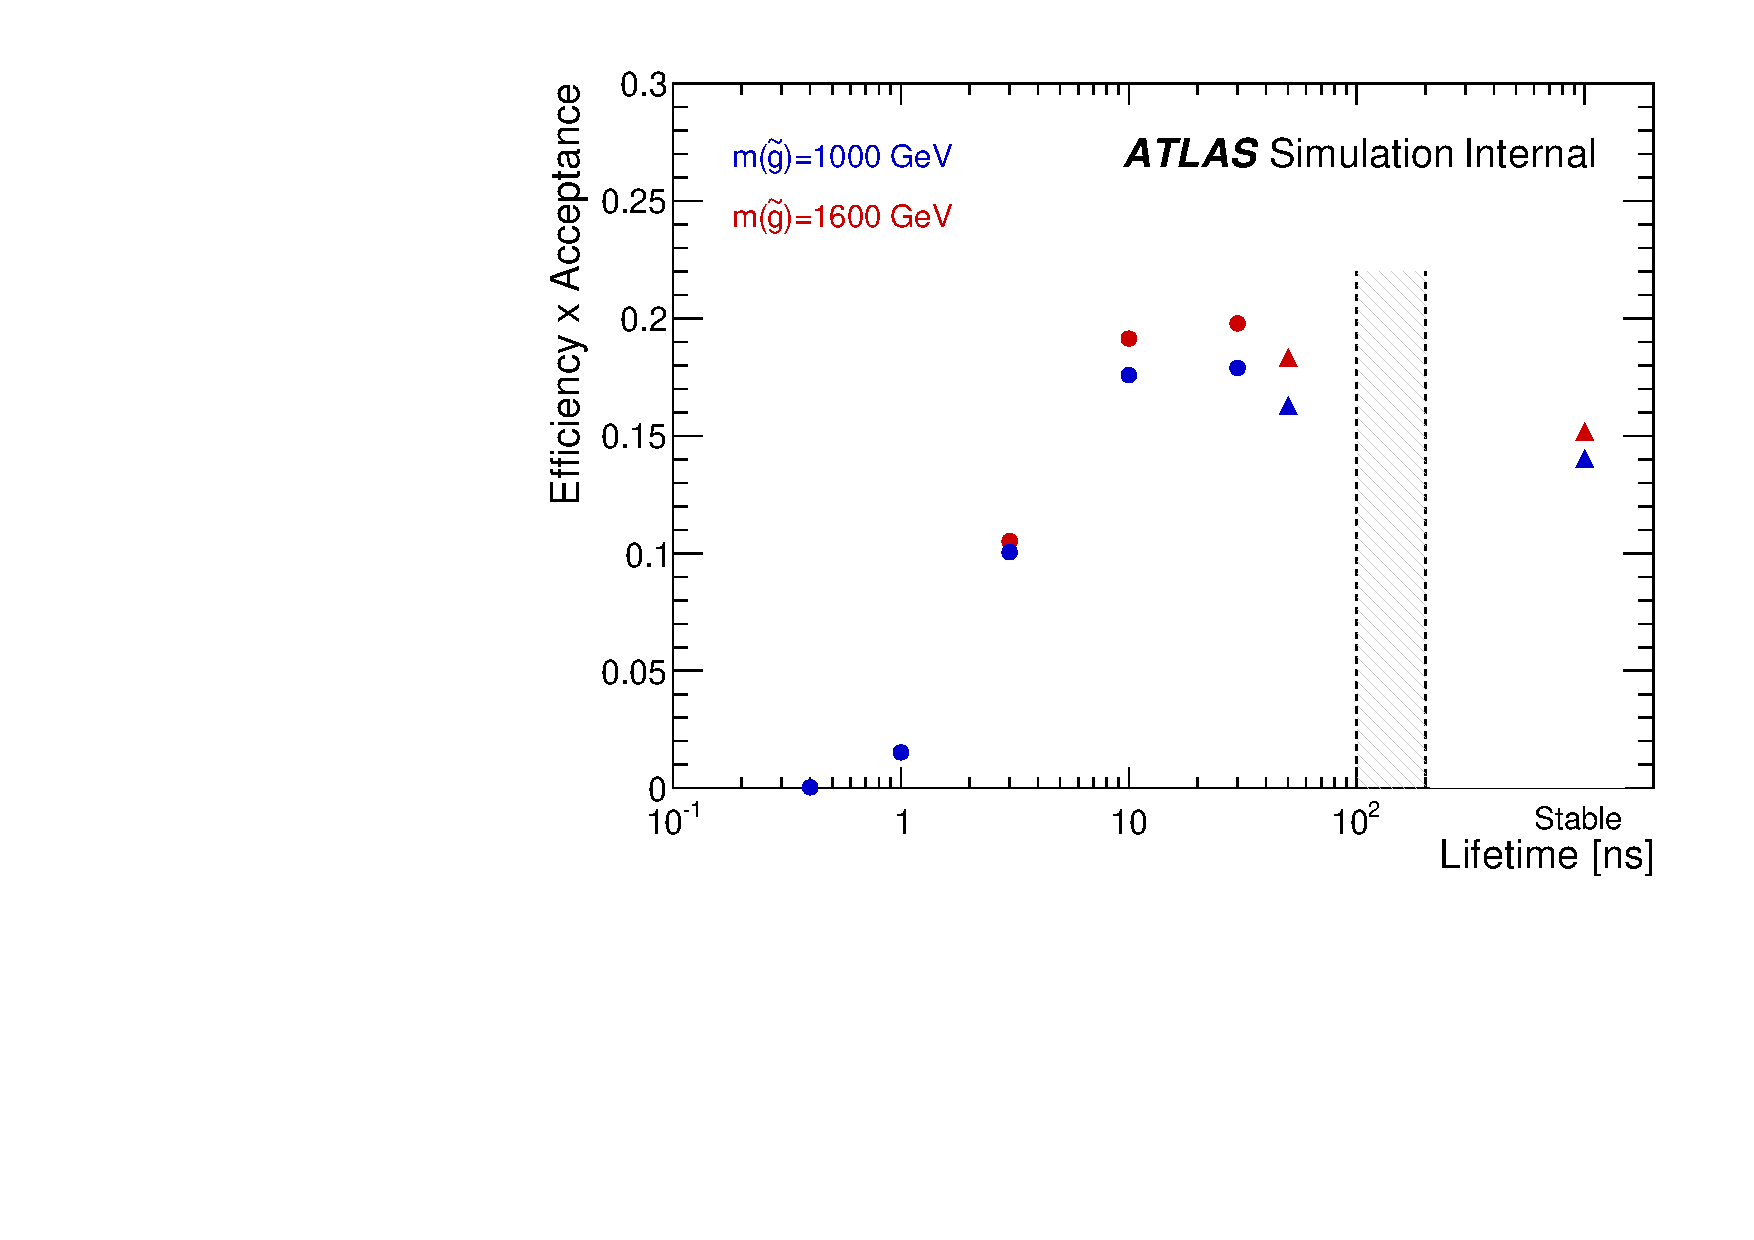
\includegraphics[width=\halffig]{figures/efficiency_lifetime.pdf}
}
\caption{The acceptance $\times$ efficiency as a function of \rhadron (a) mass and (b) lifetime. (a) shows all of the combinations of mass and lifetime considered in this search, and (b) highlights the lifetime dependence for 1000 \GeV and 1600 \GeV \rhadrons.}
\label{fig:efficiency}
\end{figure}

The inefficiency of this signal region at short lifetimes comes almost exclusively from an acceptance effect, in that the particles do not reach the necessary layers of the SCT.
This can be seen more clearly by defining a fiducial region which includes events with at least one \rhadron that is produced with non-zero charge, $\pt > 50$ \GeV, $p > 150$ \GeV, $|\eta| < 2.5$, and a decay distance greater than 37 cm in the transverse plane.
At short (1 ns) lifetimes, the acceptance into this region is as low as 4\%. 
Once this acceptance is accounted for, the selection efficiency ranges from 25\% at lifetimes of 1 ns up to 45\% at lifetimes of 10 ns. 

% ----------------------------------------
